% Fuzzing Tools And Fuzzers
 %if the chapter heading starts close to bottom of the page,
 %force a line break and remove the vertical vspace
\vspace{21.5pt}
\chapter{Embedded System, Challenges, Tools And Fuzzers}\label{sec:embedded_system}
In this chapter, the critical role of fuzzing is illuminated as a mechanism to
enhance the security and dependability of embedded systems. An initial
comparative exploration is presented, distinguishing conventional fuzzing
techniques and the unique challenges introduced when implementing fuzzing
within the context of embedded systems. This is followed by an extensive
examination of a selection of widely-used fuzzing tools and fuzzers,
assessing their operational competencies, user accessibility, efficacy, and
potential limitations. Key tools encompassed within this analysis include
AFL++~\cite{257204}, libFuzzer~\cite{libFuzze17:online}, ClusterFuzz~\cite{ClusterF90:online},
OSS-Fuzz~\cite{GitHubgo49:online}, FuzzTest~\cite{GitHubgo59:online}, and Atheris~\cite{atheris2020}. The chapter culminates with a meticulous
survey of relevant open-source initiatives and current research trajectories
within the field of fuzzing.

\section{Embedded System}

Embedded systems, which are specialized computer systems engineered for specific
tasks, diverge significantly from conventional, multi-purpose computers. These
integrated systems are composed of hardware, software, and occasionally
mechanical components, all designed to perform specific functions either
autonomously or within a larger system. In contrast to general-purpose computers,
which are designed for multitasking, embedded systems typically focus on
executing a single task or a related group of
tasks~\cite{marwedel2021embedded}~\cite{yun2022fuzzing}~\cite{Introduc26:online}.

The Figure:~\ref{fig:Embedded_System} shows the different components of embedded systems.

% \begin{figure}[ht]
%         \centering
%         \AltText{Embedded System}{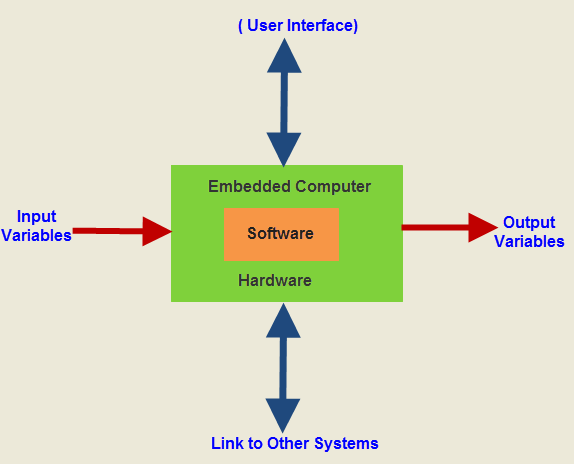
\includegraphics[width=8.5cm, height=8.5cm]{Embedded_System}}
%         \caption{Embedded System\cite{Introduc82:online}}\label{fig:Embedded_System}
% \end{figure}
\begin{figure}[h]
        \centering
        \adjustbox{width=\textwidth}{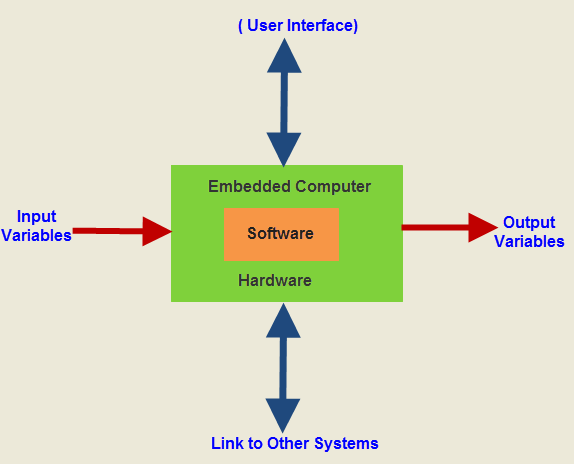
\includegraphics{Embedded_System}}
        \caption{Embedded System~\cite{Introduc82:online}}\label{fig:Embedded_System}
\end{figure}

Just like conventional computer systems, embedded systems's core components
usually include a Central Processing Unit (CPU)~\cite{WhatisaC78:online},
Random Access Memory (RAM), and input/output (I/O) interfaces. However,
embedded systems often lack user-friendly interfaces, and instead might
feature a minimal user interface or none at all~\cite{MainType35:online}.

Reflecting on the prior discussions of embedded systems and fuzzing in
Section~\ref{sec:sec_introduction} and Section~\ref{sec:sec_fuzzing} respectively,
this chapter explores further the significance and methodology of fuzzing
within the domain of embedded systems.

\subsection{Types of Embedded Devices}
Embedded systems can be classified into several types, such as standalone,
real-time, networked, and mobile systems~\cite{Classifi68:online}. These systems
play essential roles in various sectors, from consumer
electronics~\cite{andrae2010life} like digital watches~\cite{Whatisas39:online},
televisions, and cameras, to industrial machinery~\cite{thramboulidis2007soa},
medical equipment~\cite{jafari2007medical},
and automobiles~\cite{Automoti68:online}~\cite{li2003real}~\cite{MainType35:online}.

The Figure:~\ref{fig:types_of_embedded_devices} shows the different types of embedded devices.
% \begin{figure}[ht]
%         \centering
%         \AltText{Types of Embedded Devices}{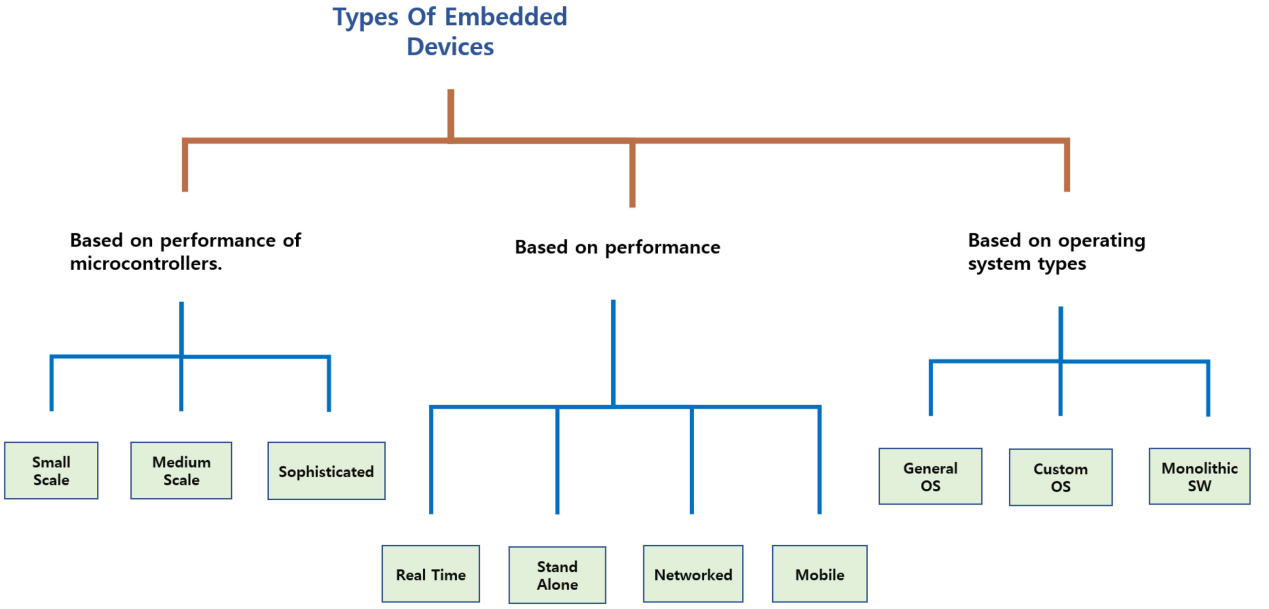
\includegraphics[width=8.5cm, height=8.5cm]{types_of_embedded_devices}}
%         \caption{Types of Embedded Devices\cite{yun2022fuzzing}\cite{WhatAreE30:online}}\label{fig:types_of_embedded_devices}
% \end{figure}

\begin{figure}[h]
        \centering
        \adjustbox{width=\textwidth}{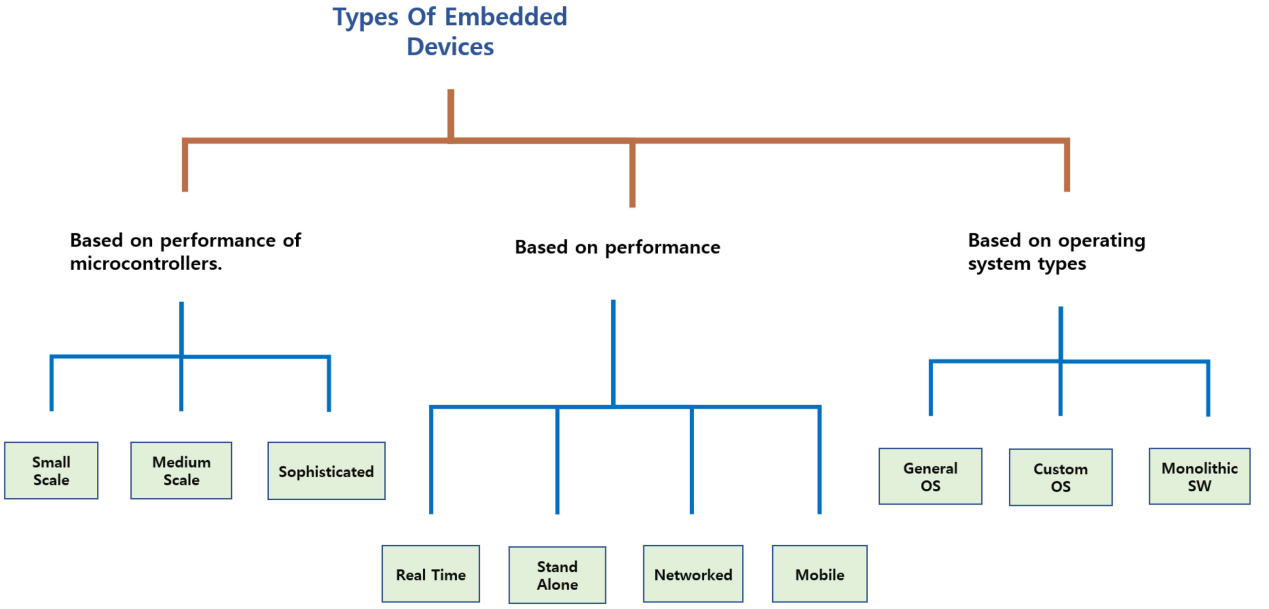
\includegraphics{types_of_embedded_devices}}
        \caption{Types of Embedded Devices~\cite{yun2022fuzzing}~\cite{WhatAreE30:online}}
        \label{fig:types_of_embedded_devices}
\end{figure}

\subsection*{Standalone Devices:}

Standalone devices constitute a subset of embedded systems functioning
independently, without the necessity for a host system. They process input data
within their own interfaces, producing outputs to control or drive attached
devices or to generate displays. These devices have found broad applicability in
various appliances due to their flexibility and efficiency. They often employ
lightweight user environments for
optimal performance~\cite{yun2022fuzzing}\cite{WhatAreE30:online}\cite{TypesofE31:online}.

\subsection*{Real-time Embedded Systems:}
Real-time embedded systems deliver outputs within specific time constraints,
crucial for timely project completion. These systems interact with external
environments via interfaces and often utilize sensors. They typically fall into
two categories: soft systems, which prioritize process completion, and hard
systems, which emphasize strict adherence to time constraints. Real-time
operating systems (RTOS) manage hardware resources and application software to
ensure task completion with precision and
consistency~\cite{Introduc22:online}\cite{yun2022fuzzing}\cite{WhatAreE30:online}\cite{TypesofE31:online}.

\subsection*{Networked embedded systems:}
Networked embedded systems form key components of wired or wireless networks,
heavily relying on web server communication. Ubiquitously found in security systems,
ATMs, and \acrlong{pos}\cite{WhatIsaP12:online} systems, these systems manage a network of devices or workstations
to perform various functions. If an embedded system forms part of or depends on a device network,
it is classified as a networked embedded
system ~\cite{Introduc22:online}~\cite{yun2022fuzzing}~\cite{WhatAreE30:online}~\cite{TypesofE31:online}.

In conclusion, the realm of embedded systems is vast and intricate,
encompassing a wide variety of devices and applications. Across these diverse
systems, there is a consistent requirement for rigorous testing and security
measures, tasks significantly streamlined by the application of fuzzing
techniques. This chapter offers an in-depth exploration of this compelling
subject, spotlighting the unique challenges and solutions in embedded
fuzzing~\cite{eisele2022embedded}. The following sections will discuss the
specific methodologies used in fuzzing for embedded systems, the challenges
encountered, and potential strategies to overcome them.


% The table:\ref{tab:embedded_devices} presents the types of embedded devices, their characteristics,
% and the challenges for fuzzing associated with each type\cite{yun2022fuzzing}.

% \begin{table}[h!]
% \centering
% \begin{tabularx}{\textwidth}{@{}>{\raggedright\arraybackslash}p{3.5cm}>{\raggedright\arraybackslash}p{3.5cm}X@{}}
% \toprule
% \textbf{Type} & \textbf{Characteristics} & \textbf{Challenges for Fuzzing} \\
% \midrule
% Standalone Devices & Own processor, memory, and peripherals; simple firmware or \acrshort{rtos}; various communication protocols & Requires specific knowledge of protocols and target hardware \\
% \addlinespace
% Devices with Embedded Linux or Other OS & Embedded version of standard OS; advanced features; higher processing power and memory capacity & Requires knowledge of OS internals and system libraries \\
% \addlinespace
% Monolithic Firmware Devices & Entire firmware in a single binary, including OS and applications & Requires full-system emulation or binary disassembly \\
% \bottomrule
% \end{tabularx}
% \caption{Types of Embedded Devices and Their Challenges for Fuzzing}
% \label{tab:embedded_devices}
% \end{table}


\subsection{Comparison Between Traditional and Embedded Fuzzing}

The Table~\ref{tab:fuzzing_comparison} provides the comparison between traditional
and embedded system fuzzing~\cite{yun2022fuzzing}~\cite{9742291}.

\begin{table}[H]
\centering
\begin{tabularx}{\textwidth}{@{}>{\raggedright\arraybackslash}p{3cm}X X@{}}
\toprule
& \textbf{Traditional Fuzzing} & \textbf{Embedded Fuzzing} \\
\midrule
\textbf{Target Systems} & Desktop and server applications, web applications, and libraries. & Real-time operating systems (RTOS), IoT devices, firmware. \\
\addlinespace
\textbf{Diverse Targets} & Server applications. & Specific hardware and protocols with limited resources and real-time constraints. \\
\addlinespace
\textbf{Challenges} & Input generation and code coverage. & Compatibility with specific hardware and operating systems. \\
\addlinespace
\textbf{Reliability Constraints} & No strict time limitations, allowing comprehensive and thorough fuzzing tests to enhance reliability of findings. & Operates under real-time constraints, demanding efficient and timely fuzzing tests. The reduced testing time could potentially affect the thoroughness and thus the reliability of the findings. \\
\addlinespace
\textbf{Testing Environment} & Simulated or actual systems with standard operating systems. & Emulators, simulators, or actual devices with specific hardware and protocols. \\
\addlinespace
\textbf{Physical Interaction} & Not a primary concern. & Required to consider environment and physical states of the system. \\
\addlinespace
\textbf{Limited Resources} & Not a primary concern. & Must optimize fuzzing tools to work efficiently within limited resources. \\
\addlinespace
\textbf{Scalability} & Can be easily parallelized to scale with the number of target applications or libraries. & Physical access to the target devices or emulators can limit scalability. \\
\addlinespace
\textbf{Tools and Techniques} & AFL, libFuzzer, Honggfuzz. & FirmFuzz, IoTcube, FUZZY. \\
\bottomrule
\end{tabularx}
\caption{Comparison of Traditional Fuzzing and Embedded Fuzzing}
\label{tab:fuzzing_comparison}
\end{table}

In addition to the general differences mentioned in the Table~\ref{tab:fuzzing_comparison}, there are more aspects to consider
when doing the comparison.

Hence, beyond the primary distinctions outlined in the Table~\ref{tab:fuzzing_comparison},
additional considerations arise when comparing traditional and embedded fuzzing techniques.
Traditional fuzzing tools typically offer a more straightforward setup than their embedded counterparts,
which may necessitate extensive manual configuration due to the wide range of
hardware and software components involved. Furthermore, integration of traditional
fuzzing into \acrlong{ci/cd} systems tends to be more straightforward,
while embedded fuzzing often requires custom solutions to accommodate
hardware specificities. Feedback in traditional fuzzing is typically
derived directly from the target application or library,
simplifying the process of monitoring fuzzing operations and
identifying anomalies. In contrast, embedded fuzzing might garner feedback
from a multitude of sources, encompassing firmware and hardware components
of the target device, which can complicate monitoring and issue detection~\cite{yun2022fuzzing}~\cite{WhatAreE30:online}.

\subsection{Challenges in Embedded Fuzzing}
Fuzz testing embedded systems presents unique challenges necessitating the
development of specialized tools and strategies to maintain system security and
reliability. This subsection discusses the primary concerns that researchers and
practitioners encounter while fuzz testing embedded systems, emphasizing the need for
inventive approaches to effectively address these issues.

\Citeauthor{yun2022fuzzing} identifies the following primary challenges:
\begin{itemize}
\item \textbf{Heterogeneous targets:} The variability in hardware, operating systems, and communication protocols in embedded systems presents a significant challenge~\cite{yun2022fuzzing}.
\item \textbf{Limited resources:} The restricted processing power and memory typically characteristic of embedded systems can limit the applicability of traditional fuzzing techniques~\cite{yun2022fuzzing}.
\item \textbf{Real-time and reliability constraints:} Some embedded systems have strict real-time requirements, and fuzzing must not interfere with their regular operations~\cite{yun2022fuzzing}.
\item \textbf{Scalability issues:} Fuzzing often requires physical access to target devices or emulators, which can impede scalability~\cite{yun2022fuzzing}.
\end{itemize}

~\Citeauthor{muench2018you} highlights further obstacles:
\begin{itemize}
\item \textbf{Limited visibility:} The internal state of embedded systems is often difficult to observe, complicating the interpretation of fuzz testing impacts and issue identification~\cite{muench2018you}.
\item \textbf{Reproduction of crashes:} The diverse nature of embedded systems and the use of custom hardware may hinder the consistent and accurate reproduction of crashes~\cite{muench2018you}.
\item \textbf{Root cause analysis:} There exist difficulties in discerning the root cause of crashes in embedded systems~\cite{muench2018you}.
\end{itemize}

~\Citeauthor{eisele2022embedded} enumerates additional complexities:
\begin{itemize}
\item \textbf{Physical interaction:} Embedded systems often interact with the physical world, further complicating fuzzing tasks~\cite{eisele2022embedded}.
\item \textbf{Device-specific hardware and protocols:} Custom hardware components and communication protocols in embedded devices may not be compatible with existing fuzzing tools and techniques~\cite{eisele2022embedded}.
\item \textbf{Lack of source code:} Absence of source code for embedded systems can hinder software analysis for potential vulnerabilities and hamper the development of appropriate fuzzing test cases~\cite{eisele2022embedded}.
\end{itemize}

~\Citeauthor{manes2019art} discusses the following challenges:
\begin{itemize}
\item \textbf{Stateful applications:} Fuzzing stateful applications, such as network protocols or multi-threaded applications, necessitates effective handling of state transitions, synchronization, and concurrent execution~\cite{manes2019art}.
\item \textbf{Oracle problem:} Identifying whether a specific input has triggered a vulnerability can pose challenges. Fuzzers often depend on simple oracles like crashes, which may not be sufficient for detecting all types of vulnerabilities~\cite{manes2019art}.
\item \textbf{Performance:} The efficiency of fuzzers is critical for their efficacy. Slow fuzzers may not explore sufficient execution paths within a reasonable timeframe, thus failing to uncover vulnerabilities~\cite{manes2019art}.
\end{itemize}

\section{Fuzzing Tools and Fuzzers}

Fuzzing embedded systems presents unique challenges and requirements, necessitating the development
of dedicated tools and techniques. This section provides an overview of several fuzzing tools,
their functionality, ease of use, and their advantages and limitations.

\begin{longtable}{p{2.5cm}p{3cm}p{3cm}p{5cm}}
\caption{Different Types of Fuzzers}
\label{tab:fuzzers_table} \\
\toprule
\textbf{Name} & \textbf{Functionality} & \textbf{Ease of use} & \textbf{Effectiveness and Limitations} \\
\midrule
\endfirsthead
\toprule
\textbf{Name} & \textbf{Functionality} & \textbf{Ease of use} & \textbf{Effectiveness and Limitations} \\
\midrule
\endhead
AFL~\cite{zalewski2014american}~\cite{GitHubgo92:online} & Coverage-guided, genetic algorithms, binary program fuzzing & Simple setup, easy to use & Widely adopted, has discovered numerous vulnerabilities. Lacks support for multi-threaded applications, and limited effectiveness in fuzzing structured data formats \\
\midrule
libFuzzer~\cite{libFuzze17:online} & Coverage-guided, in-process fuzzing, targets libraries with well-defined APIs & Easy integration with LLVM-based projects, requires writing custom harness code & Has found vulnerabilities in widely-used libraries and software components. In-process fuzzing can result in performance bottlenecks, limited support for non-LLVM compilers \\
\midrule
honggfuzz~\cite{GitHubgo89:online} & Security-oriented, supports multiple platforms and feedback signals & Moderate setup complexity, flexible configuration options & Effective in identifying vulnerabilities in various types of software. Lacks the ease of use and setup simplicity compared to AFL, limited documentation \\
\midrule
Boofuzz\cite{pereyda2019boofuzz} & Network protocol fuzzing, custom protocol specifications & Moderate setup complexity, flexible configuration options & Effective in finding vulnerabilities in network protocols and services. Limited support for non-network protocol targets, can be complex to configure for custom protocols \\
\midrule
Radamsa~\cite{AkiHelin96:online} & Black-box fuzzer for file formats, network protocols, and command-line utilities & Simple to use for black-box testing scenarios & Has identified vulnerabilities in a wide range of software. Lacks feedback-driven fuzzing capabilities, limited in identifying complex vulnerabilities \\
\midrule
AFL++~\cite{257204} & Enhanced version of AFL with improved mutation strategies and performance & Similar to AFL, simple setup, and easy to use for most users & Inherits AFL's effectiveness and adds various improvements. Still inherits some limitations of AFL, such as the lack of support for multi-threaded applications and structured data formats \\
\midrule
FirmFuzz~\cite{srivastava2019firmfuzz}~\cite{yun2022fuzzing}  & Automated IoT firmware introspection and analysis & Requires understanding of firmware images and emulation & Useful for identifying vulnerabilities in firmware images. Limited to firmware images, requires specific knowledge and expertise in firmware analysis \\
\midrule
Firmadyne~\cite{chen2016towards} & Emulation and dynamic analysis of Linux-based embedded firmware & Moderate setup complexity, requires knowledge of firmware and Linux systems & Effective in analyzing firmware for potential vulnerabilities. Limited to Linux-based firmware, emulation may not accurately represent the actual hardware environment \\
\midrule
AVATAR~\cite{zaddach2014avatar}  & Framework for dynamic analysis and instrumentation of embedded systems & Requires understanding of embedded systems and experience with dynamic analysis & Can be effective when combined with fuzzers for analyzing embedded firmware. Steep learning curve, requires customization for specific target systems \\
\midrule
Atheris~\cite{GitHubgo74:online} & Coverage-guided, native and Python fuzzer with integration with libFuzzer & Easy to use, Python script fuzzing & Effective in identifying vulnerabilities in Python and native extensions. Requires Python 3.3 or later, and it is mostly tested on Linux \\
\bottomrule
\end{longtable}

\section{Open-source Projects and Ongoing Research} This section examines
open-source projects and ongoing research in the realm of fuzzing. The
effectiveness of security testing in revealing vulnerabilities in software
systems has gained prominence in recent years due to the discovery of
high-profile bugs. The Heartbleed bug~\cite{Heartble53:online}, discovered in
OpenSSL in 2014, and the Shellshock bug~\cite{shetty2018shellshock}, found in the
Bash shell in the same year, serve as critical examples of vulnerabilities with
widespread impacts on the internet. Although not uncovered through fuzzing,
their discovery emphasized the necessity of thorough security testing.
Section~\ref{par:success_of_fuzzing} details the accomplishments and
vulnerabilities unveiled by fuzzing techniques over time.

This discussion highlights several notable open-source fuzzing initiatives,
including Google's OSS-Fuzz~\cite{GitHubgo49:online}, a variety of AFL-based
fuzzers~\cite{257204}, and a GitHub repository dedicated to fuzzing research. The
primary objective of these projects is to expand the current capabilities of
fuzzing. They aim to provide a collaborative platform that fosters knowledge
sharing among the fuzzing community.

The exploration of these open-source projects and the active research in
fuzzing offered in this section aims to impart valuable insights into the
current trends and potential future directions of fuzzing as a vital tool in
software security testing.

\textbf{OSS-Fuzz:~\cite{GitHubgo49:online}} \\

Google's OSS-Fuzz represents a pioneering initiative in the domain of open-source fuzzing.
Its uniqueness lies not merely in its goal of enhancing security and stability—which is indeed a
common objective across all fuzzing projects—but in its commitment to continuous,
automated fuzzing for selected open-source software projects.

OSS-Fuzz stands out in its adaptability, integrating with a variety of fuzzing engines such as
libFuzzer~\cite{libFuzze17:online} and AFL++~\cite{257204}.
Furthermore, it supports multiple programming languages, demonstrating its versatility in accommodating
projects written in C, C++, Rust~\cite{klabnik2023rust}, and Go~\cite{donovan2015go}. This broad compatibility reinforces its value to the diverse
landscape of open-source software~\cite{ShortInt96:online}.

\textbf{OneFuzz:~\cite{GitHubmi60:online}}\\

The OneFuzz~\cite{GitHubmi60:online} is a fuzzing-as-a-service platform developed by Microsoft, that aims to
automate the detection and reporting of software bugs. It is a self-hosted
platform that provides a range of features, including task scheduling,
crash analysis, and distributed fuzzing. OneFuzz can be integrated with
existing development workflows, making it a useful tool for organizations
looking to improve the security and stability of their software systems

\textbf{Afl Based Fuzzers:}\\

\acrlong{afl}~\cite{american20:online} is a coverage-guided~\cite{lyu2022ems}, or feedback-based fuzzer that utilizes a
dynamic approach to identify potential vulnerabilities in software applications.
It modifies the target executable to measure and optimize code coverage,
mutating input data in a manner that maximizes the coverage achieved.
This process is iteratively repeated, seeking to uncover instances in
which the program crashes, thereby identifying potential security vulnerabilities.
AFL has proven to be highly effective in practice, as evidenced by its extensive
usage and success in uncovering numerous vulnerabilities in widely-used software.
Furthermore, AFL is renowned for its ease of use, making it a popular choice
among security researchers and practitioners~\cite{american20:online}~\cite{fuzzinga40:online}.

Several fuzzers have been developed based on AFL's architecture~\cite{american20:online}, enhancing its
capabilities or tailoring it for specific use cases. Some notable AFL-based
fuzzers mentioned below:

\textbf{AFL++:~\cite{257204}~\cite{GitHubAF78:online}} \\
An enhanced version of AFL which
introduces various performance improvements and new features, such as improved mutation strategies,
faster execution, more and better mutations, improved instrumentation, and custom module
support~\cite{257204}~\cite{GitHubAF78:online}.

\textbf{AFLFast:~\cite{GitHubmb97:online}} \\
A fuzzer that introduces a power schedule, aiming to prioritize
seeds that are more likely to explore new paths and increase coverage.
By doing so, the AFLFast~\cite{GitHubmb97:online} aims to improve the efficiency of fuzzing and maximize
the code coverage in a shorter time frame~\cite{bohme2016coverage}~\cite{GitHubmb97:online}.

\textbf{TriforceLinuxSyscallFuzzer:~\cite{GitHubnc62:online}} \\

This fuzzing technique specifically targets Linux system calls,
aiming to identify potential vulnerabilities in the system call interface\cite{GitHubnc62:online}.

\textbf{AFL-unicorn:~\cite{GitHubBa48:online}} \\

AFL-Unicorn~\cite{GitHubBa48:online} represents a noteworthy extension of the American Fuzzy Lop (AFL) framework,
characterized by its versatility across various architectures, data input formats, and
binary formats—including the firmware~\cite{WhatIsFi49:online} of bare-metal devices
such as Wi-Fi components and baseband~\cite{Baseband1:online} processors in mobile phones.
This utility is designed to examine binary files and then create a fuzzer that
emulates the state at the entry point of the parsing routine.

The efficacy of AFL-Unicorn is underpinned by the successful integration of
AFL's coverage-guided fuzzing technique and the~\cite{Unicorn–92:online} engine.
This synergistic combination facilitates the exploration of multiple execution
paths within the targeted binary, including those within proprietary,
closed-source firmware like that running on baseband processors~\cite{tell2005design}. This capability
contributes to a thorough and comprehensive fuzzing process, even in the context
of complex and traditionally opaque systems~\cite{maier2019unicorefuzz}~\cite{aflunico82:online}.
\clearpage